\documentclass[aspectratio=169,11pt]{beamer}

\usepackage{graphicx}
\usepackage{tikz}
\usetikzlibrary{positioning,arrows.meta}
\usepackage{xcolor}
\usepackage{booktabs}
\usepackage{tabularx}
\usepackage{array}
\usepackage{ragged2e}

\definecolor{GEUBlue}{RGB}{20,55,105}
\definecolor{GEULightBlue}{RGB}{238,244,251}
\definecolor{GEUGrey}{RGB}{90,90,90}
\definecolor{GEULightGrey}{RGB}{245,246,248}

\usetheme{default}
\setbeamertemplate{navigation symbols}{}
\setbeamertemplate{blocks}[rounded][shadow=false]
\setbeamercolor{normal text}{fg=black,bg=white}
\setbeamercolor{frametitle}{fg=GEUBlue}
\setbeamercolor{structure}{fg=GEUBlue}
\setbeamercolor{block title}{fg=GEUBlue,bg=GEULightBlue}
\setbeamercolor{block body}{fg=black,bg=GEULightBlue}
\setbeamerfont{frametitle}{size=\Large,series=\bfseries}

% Replace with the actual logo filename
\newcommand{\GEULogo}{logo.png}

% Header and footer
\setbeamertemplate{headline}{%
  \begin{tikzpicture}[remember picture,overlay]
    \node[anchor=north east,xshift=-0.30cm,yshift=-0.12cm]
      at (current page.north east)
      {\includegraphics[height=0.62cm]{\GEULogo}};
  \end{tikzpicture}
  \vspace{0.72cm}
}
\setbeamertemplate{frametitle}{%
  \vspace{0.03cm}
  \insertframetitle\par
  \vspace{0.04cm}
  \textcolor{GEUBlue}{\rule{\textwidth}{0.9pt}}
  \vspace{0.03cm}
}
\setbeamertemplate{footline}{%
  \leavevmode
  \hbox{%
  \begin{beamercolorbox}[wd=.82\paperwidth,ht=0.32cm,dp=0.10cm,leftskip=.3cm]{author in head/foot}
    \tiny Department of Computer Science \& Engineering | Graphic Era (Deemed to be University)
  \end{beamercolorbox}%
  \begin{beamercolorbox}[wd=.18\paperwidth,ht=0.32cm,dp=0.10cm,rightskip=.3cm]{date in head/foot}
    \hfill\tiny\insertframenumber/\inserttotalframenumber
  \end{beamercolorbox}}
}

\newcommand{\smallnote}[1]{\vspace{0.08cm}{\scriptsize\color{GEUGrey}#1}}

\title{\textbf{Project-Based Learning}\\[2mm]\large Phase-III Final Evaluation}
\author{\textbf{RideSync: A Graph-Based Smart Cab Booking and Dispatch Simulation System}\\Team ID: DSCPP-III-2026-T151}
\institute{Department of Computer Science \& Engineering\\Graphic Era (Deemed to be University), Dehradun}
\date{Academic Session 2026--27}

\begin{document}

% 1. Title Slide
\begin{frame}[plain]
\begin{tikzpicture}[remember picture,overlay]
\draw[GEUBlue,line width=3pt] (current page.north west) -- (current page.north east);
\node[anchor=north east,xshift=-0.45cm,yshift=-0.35cm] at (current page.north east)
{\includegraphics[height=1.0cm]{\GEULogo}};
\node[align=center,text width=.84\paperwidth] at ([yshift=.25cm]current page.center)
{{\color{GEUBlue}\fontsize{24}{28}\selectfont\bfseries PROJECT-BASED LEARNING}\\[2mm]
 {\fontsize{16}{20}\selectfont PHASE-III FINAL EVALUATION}\\[5mm]
 {\color{GEUGrey}\large\bfseries RideSync: A Graph-Based Smart Cab Booking and Dispatch Simulation System}\\[2mm]
 {\color{GEUBlue}\small Team ID: DSCPP-III-2026-T151}};
\node[align=center,anchor=south,yshift=.42cm] at (current page.south)
{\bfseries Department of Computer Science \& Engineering\\
Graphic Era (Deemed to be University), Dehradun\\[-1mm]
\scriptsize Academic Session 2026--27};
\end{tikzpicture}
\end{frame}

% 2. Team & Mentor Details
\begin{frame}{Team \& Mentor Details}
\small
\vspace{-2mm}
\begin{columns}[T,totalwidth=\textwidth]

\column{.48\textwidth}
\begin{block}{Team Information}
\begin{tabular}{@{}p{2.2cm}p{4.3cm}@{}}
\textbf{Team ID:} & DSCPP-III-2026-T151\\
\textbf{Semester:} & 3rd\\
\textbf{Team Name:} & The Four Bytes\\
\textbf{Domain:} & Data Structures and
                 \\& Programming in C++
\end{tabular}
\end{block}

\column{.48\textwidth}
\begin{block}{Team Members}
\footnotesize
1.\quad Gupta, Tanvi -- 2510010362 (Lead)\\
2.\quad Jahnavi -- 2510380066\\
3.\quad Tyagi, Nishtha -- 2510370096\\
4.\quad Sharma, Dhairya -- 2510011490
\end{block}

\end{columns}

\vspace{1mm}

\begin{block}{Mentor}
\footnotesize
\textbf{Dr.Hemant Singh Pokhariya (hemantsinghpokhariya@geu.ac.in)}
\hfill
\textbf{Interactions completed: 8}\\
\textbf{submitted to : Ms. Nishtha Bhatt, Mr. Ramesh Singh Rawat.}

\end{block}

\end{frame}

% 3. Phase-III Abstract & Updated Approach
\begin{frame}{Phase-III Abstract \& Final System Approach}

\vspace{-3mm}

\begin{block}{Project Abstract}
\scriptsize
RideSync is a full-stack smart cab booking and dispatch simulation system. The core backend logic is implemented in C++17 utilizing weighted graph models, Dijkstra's algorithm for shortest routes, priority queue driver scoring, and persistence. An interactive web UI connected to a Node.js REST API server provides seamless end-to-end user and driver workflows.
\end{block}

\vspace{0.6mm}

\begin{columns}[T,totalwidth=\textwidth]

\column{.60\textwidth}
\textbf{\color{GEUBlue}Architecture Highlights}
\begin{itemize}\itemsep1pt
\item \footnotesize Encapsulated C++ OOP classes: Customer, Driver, Cab, Admin, Booking
\item \footnotesize Full Web UI: \texttt{index.html}, \texttt{style.css}, \texttt{app.js}
\item \footnotesize Node.js REST API server (\texttt{server.js}) with JSON persistence
\item \footnotesize Weighted Graph \& Dijkstra Shortest Path Engine
\item \footnotesize STL \texttt{std::stack} for recent user booking history
\end{itemize}

\column{.45\textwidth}
\textbf{\color{GEUBlue}Design Choices}
\begin{itemize}\itemsep1pt
\item \footnotesize Modular separation: Header (\texttt{.hpp}), Source (\texttt{.cpp}), Web static assets
\item \footnotesize Dual-tier execution: Standalone C++ engine \& Node.js Web backend
\item \footnotesize Priority Queue max-heap driver assignment based on composite score
\item \footnotesize Robust validation against invalid node IDs and unavailable cabs
\end{itemize}

\end{columns}

\end{frame}

% 4. Tasks Completed in Phase-III
\begin{frame}{Phase-III Progress: Tasks Completed}

\footnotesize
\vspace{-2mm}
\textbf{\color{GEUBlue}Final Completed Milestones \& Contributions}
\vspace{1mm}

\begin{itemize}\itemsep2pt
\item \textbf{Graph Representation \& Routing Engine:} City graph adjacency list and Dijkstra's algorithm fully implemented by Jahnavi.
\item \textbf{Priority-Queue Driver Dispatch:} Max-heap ranking based on physical distance and driver rating completed by Dhairya Sharma.
\item \textbf{Booking Lifecycle \& Dynamic Fares:} Complete booking state machine and distance-based fare calculation implemented by Tanvi Gupta \& Nishtha Tyagi.
\item \textbf{Web UI \& REST API Backend:} Modern responsive web interface and Node.js server created and deployed by Tanvi Gupta.
\item \textbf{File Handling \& Persistence:} JSON \& file-based persistence for users, rides, and logs by Dhairya Sharma \& Nishtha Tyagi.
\item \textbf{System Integration \& Core Testing:} End-to-end integration and automated unit testing (\texttt{test\_core.cpp}) completed by All Team Members.
\end{itemize}

\end{frame}

% Full-page image slide
\begin{frame}[plain]
    \centering
    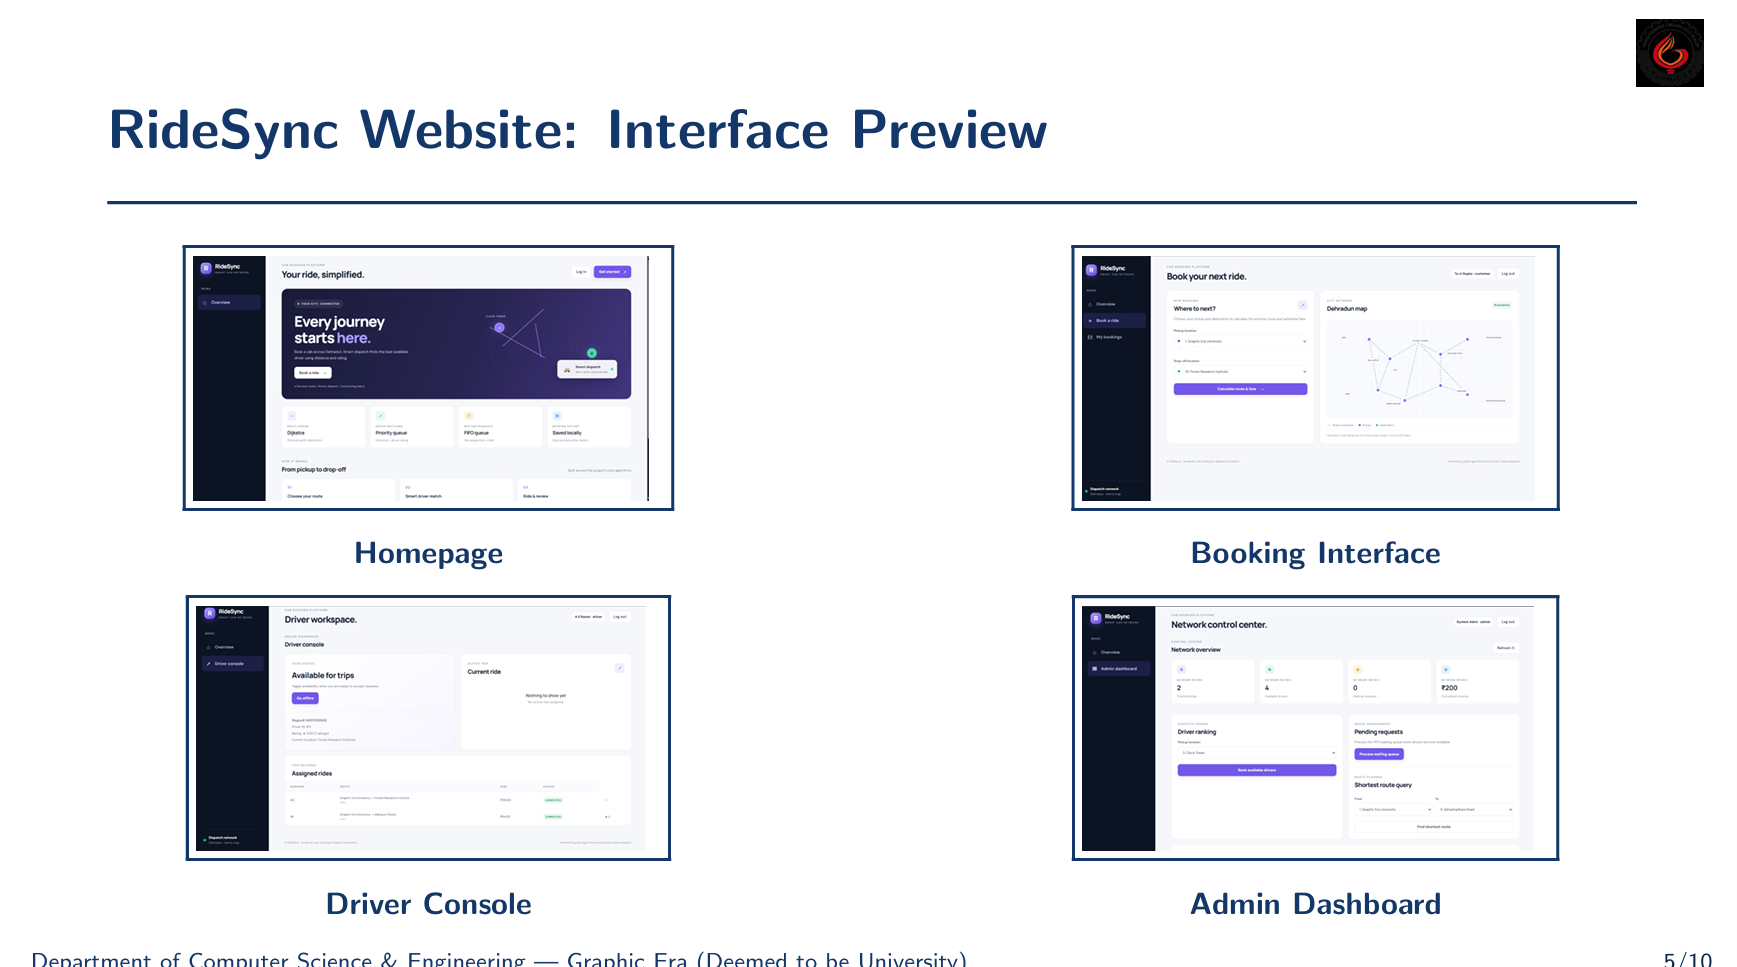
\includegraphics[width=\paperwidth,height=\paperheight]{image.png}
\end{frame}

% 5. Challenges & Technical Roadblocks Addressed
\begin{frame}{Challenges \& Technical Solutions}

\footnotesize
\vspace{-2mm}

\begin{columns}[T,totalwidth=\textwidth]

\column{.48\textwidth}
\textbf{\color{GEUBlue}Challenges Encountered}
\begin{enumerate}\itemsep1pt
\item \textbf{Module Integration:} Coordinating seamless integration across C++ STL modules and Node.js API endpoints.
\item \textbf{Edge Case Validation:} Handling network disconnects, unavailable drivers, and invalid route inputs gracefully.
\item \textbf{State Persistence:} Keeping file/JSON storage consistent across web sessions and application restarts.
\end{enumerate}

\column{.48\textwidth}
\textbf{\color{GEUBlue}Solutions Implemented}
\begin{enumerate}\itemsep1pt
\item \textbf{Composite Dispatch Scoring:} Formulated weighted max-heap algorithm combining distance and driver rating.
\item \textbf{Automated Core Testing:} Implemented \texttt{test\_core.cpp} to validate routing, assignment, and fares before integration.
\item \textbf{Unified API Layer:} Clean REST API in \texttt{server.js} interfacing web frontend directly with data structures.
\end{enumerate}

\end{columns}

\vspace{2mm}
\begin{center}
\tiny
\textit{Repository: \texttt{github.com/TanviGupta12/RideSync-Cab-Booking-Dispatch} (Branch: \texttt{main})} \\
\textit{Website: \texttt{https://ridesync-cab-booking-dispatch.onrender.com}}
\end{center}

\end{frame}

% 6. Integration of PBL Course Concepts
\begin{frame}{Integration of PBL Course Concepts}
\tiny
\begin{center}
\renewcommand{\arraystretch}{1.2}
\begin{tabularx}{.96\textwidth}{@{}>{\bfseries}p{3.5cm}X p{2.2cm}@{}}
\toprule
Course/Area & Concepts Applied & Project Module\\
\midrule
Data Structures \& Algorithms & Graph Adjacency List, Priority Queue Max-Heap, Stack, Dijkstra's Algorithm, Sorting & City Routing, Driver Dispatch, Booking History\\
OOP with C++ & Classes \& Objects, Constructors, Inheritance, Polymorphism, Encapsulation, STL, File Stream & Customer, Driver, Cab, Admin, Booking System\\
Web & REST API, Asynchronous JS, Flexbox/Grid CSS, JSON Storage & Frontend UI (\texttt{app.js}) \& Backend Server (\texttt{server.js})\\
\bottomrule
\end{tabularx}
\end{center}

\vspace{2mm}

\begin{center}
\colorbox{GEULightBlue}{\parbox{.86\textwidth}{\centering
\scriptsize \textbf{Final Update:} Successfully combined advanced C++ STL containers (\texttt{vector}, \texttt{priority\_queue}, \texttt{unordered\_map}, \texttt{stack}) and OOP design patterns with a responsive web architecture.}}
\end{center}
\end{frame}

% 7. Codebase & Component Status
\begin{frame}{Codebase \& Final Component Status}

\vspace{-4mm}

\begin{center}
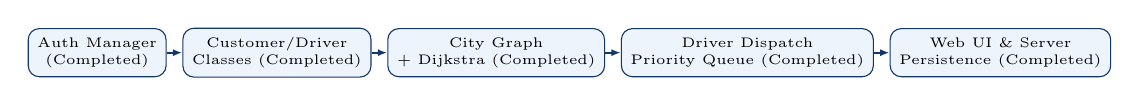
\begin{tikzpicture}[
node distance=2mm,
box/.style={
rectangle,
rounded corners,
draw=GEUBlue,
fill=GEULightBlue,
minimum width=1.5cm,
minimum height=6mm,
align=center,
font=\tiny
},
arrow/.style={
-{Latex[length=1.2mm]},
thick,
draw=GEUBlue
}
]

\node[box] (a) {Auth Manager\\(Completed)};
\node[box,right=of a] (b) {Customer/Driver\\Classes (Completed)};
\node[box,right=of b] (c) {City Graph\\+\ Dijkstra (Completed)};
\node[box,right=of c] (d) {Driver Dispatch\\Priority Queue (Completed)};
\node[box,right=of d] (e) {Web UI \& Server\\Persistence (Completed)};

\draw[arrow] (a)--(b);
\draw[arrow] (b)--(c);
\draw[arrow] (c)--(d);
\draw[arrow] (d)--(e);

\end{tikzpicture}
\end{center}

\vspace{0mm}

\begin{columns}[T,totalwidth=\textwidth]

\column{.48\textwidth}
\textbf{\color{GEUBlue}\tiny Key Contributions \& Commits}
\begin{itemize}\itemsep0.5pt
\item \tiny \textbf{Tanvi Gupta:} Architecture, Auth, dynamic fares, Web UI, CLI
\item \tiny \textbf{Jahnavi:} CityGraph adjacency list \& Dijkstra routing engine
\item \tiny \textbf{Nishtha Tyagi:} Derived user classes, location tracking, stack history
\item \tiny \textbf{Dhairya Sharma:} Priority Queue driver scoring, File logging, Node.js REST server
\end{itemize}

\column{.48\textwidth}
\textbf{\color{GEUBlue}\tiny Testing \& Validation Status (100\% PASSED)}
\begin{itemize}\itemsep0.5pt
\item \tiny \textbf{Unit Testing (\texttt{test\_core.cpp}):} PASSED (Graph, Dispatch, Auth, Booking)
\item \tiny \textbf{Input Validation:} PASSED (Invalid node IDs, out-of-service cabs handled)
\item \tiny \textbf{Integration Testing:} PASSED (End-to-end CLI \& Web API verified)
\end{itemize}

\end{columns}

\end{frame}

% 8. Technology Stack & Methodology
\begin{frame}{Technology Stack \& Final Methodology}

\footnotesize
\vspace{-3mm}

\begin{columns}[T,totalwidth=\textwidth]

\column{.55\textwidth}
\begin{block}{Technology Stack}
\tiny
\begin{itemize}\itemsep0.5pt
\item Core Language: C++17 (GCC/Clang, Makefile)
\item STL Containers: \texttt{vector}, \texttt{queue}, \texttt{priority\_queue}, \texttt{unordered\_map}, \texttt{stack}
\item Algorithms: Dijkstra's Shortest Path, Max-Heap Priority Dispatch
\item Web Stack: HTML5, CSS3, JavaScript (ES6+), Node.js HTTP/Crypto
\item Storage: Flat files (\texttt{fstream}) \& \texttt{data/ridesync.json}
\item Build Tools: Makefile, VS Code, Git/GitHub
\end{itemize}
\end{block}

\column{.41\textwidth}
\begin{block}{Development Methodology}
\tiny
\begin{enumerate}\itemsep0.5pt
\item Problem Definition 
\item Requirement Analysis 
\item System Design 
\item Class Design \& Auth 
\item Algorithm Integration 
\item Web \& File Persistence 
\item Testing \& Final Deployment 
\end{enumerate}
\end{block}

\end{columns}

\end{frame}

% 9. Final Deliverables & Summary
\begin{frame}{Final Project Deliverables \& Summary}

\tiny
\vspace{-5mm}

\begin{columns}[T,totalwidth=\textwidth]

\column{.64\textwidth}
\textbf{\color{GEUBlue}Completed Tasks Summary}

\begin{enumerate}
\setlength{\itemsep}{0.5pt}
\setlength{\parskip}{0pt}
\item \textbf{Graph Representation \& Dijkstra Routing:} Jahnavi

\item \textbf{Priority-Queue Driver Assignment:} Dhairya Sharma
\item \textbf{Booking System \& Fare Calculation:} Tanvi Gupta \& Nishtha Tyagi 
\item \textbf{File Persistence \& Log Storage:} Tanvi Gupta \& Nishtha Tyagi 
\item \textbf{Web UI \& Node.js API Deployment:} Dhairya Sharma 
\item \textbf{System Integration \& End-to-End Testing:} All Team Members 
\end{enumerate}

\vspace{1mm}

\textbf{\color{GEUBlue}Execution Roadmap Status}

\begin{enumerate}
\setlength{\itemsep}{0.5pt}
\setlength{\parskip}{0pt}
\item Phase 1: Requirements \& Architectural Design (\textit{Completed})
\item Phase 2: OOP Structure, C++ Data Structures \& Auth (\textit{Completed})
\item Phase 3: Web UI, REST Server, Integration \& Testing (\textit{Completed})
\end{enumerate}

\column{.34\textwidth}
\textbf{\color{GEUBlue}References}

\begin{enumerate}
\setlength{\itemsep}{0.5pt}
\setlength{\parskip}{0pt}
\item cppreference.com -- C++17 Standard
\item Node.js v18+ HTTP \& Crypto APIs
\item GeeksforGeeks -- Dijkstra's Algorithm
\item GeeksforGeeks -- Priority Queue Max-Heap
\item GitHub Repository: \texttt{TanviGupta12/RideSync-Cab-Booking-Dispatch}
\end{enumerate}

\vspace{2mm}

\begin{center}
\colorbox{GEUBlue}{%
\parbox{.98\linewidth}{%
\centering
\color{white}
\textbf{Thank You!}\\[-1pt]
RideSync System Complete
}}
\end{center}

\end{columns}

\end{frame}

\end{document}